\chapter{Çoklu Doğrusal Regresyon; Ayarlanmış İlişkiler, Karıştırıcılık ve Etkileşim}
\label{ch:multiple-regression}

\begin{hedefler}
Bu bölümün sonunda:
\begin{itemize}
  \item çoklu doğrusal regresyon katsayılarını diğer açıklayıcılar sabitken yorumlayabilecek,
  \item kategorik açıklayıcıları gösterge değişkenlerle modele katabilecek,
  \item karıştırıcılık, etkileşim ve çoklu bağlantı kavramlarını birbirinden ayırabilecek,
  \item model uyumunu, katsayı belirsizliğini ve artık tanılarını birlikte değerlendirebileceksiniz.
\end{itemize}
\end{hedefler}

\begin{prerequisitebox}
Basit doğrusal regresyon, korelasyon, eğim, güven aralığı, \pval-değeri, artık ve
$R^2$ kavramları bilinmelidir. Kategorik ve nicel değişken ayrımı
hatırlanmalıdır.
\end{prerequisitebox}

\begin{hazirlik}
Çalışma süresi ile başarı arasındaki ilişki, önceki başarı modele eklendiğinde
neden değişebilir? ``Kontrol etmek'' ile nedensel etkiyi kanıtlamayı ayırın.
\end{hazirlik}

Basit regresyon eğimi, $R^2$ ve artık tanıları Bölüm~\ref{ch:correlation-regression}'de
verilmiştir. Bu bölüm aynı yapıyı birden fazla açıklayıcı değişkene genişletir.

\section{Neden birden fazla açıklayıcı değişken?}

Eğitim sonuçları çoğu zaman tek bir değişkenle açıklanamaz. Başarı puanı;
çalışma süresi, önceki başarı, devamsızlık, öğretim yöntemi ve okul kaynakları
gibi birbiriyle ilişkili birçok değişkene bağlı olabilir. Basit regresyon iki
değişken arasındaki toplam ilişkiyi gösterirken çoklu regresyon, bir
açıklayıcının diğer modele alınmış değişkenler sabitken taşıdığı ilişkiyi
inceler. Katsayı yorumu, model kurma ve tanı ilkeleri için
\citet{gelman2020}, \citet{fox2016} ve \citet{james2021} temel başvuru
kaynaklarıdır.

Çoklu doğrusal model
\[
Y_i=\beta_0+\beta_1X_{1i}+\beta_2X_{2i}+\cdots+
\beta_KX_{Ki}+\varepsilon_i
\]
biçimindedir. Uydurulan modelde bilinmeyen parametrelerin yerini örneklem
katsayıları alır:
\[
\hat Y_i=b_0+b_1X_{1i}+b_2X_{2i}+\cdots+b_KX_{Ki}.
\]

\begin{definitionbox}
\textbf{Çoklu doğrusal regresyon}, nicel bir yanıtın koşullu ortalamasını
birden fazla açıklayıcı değişkenin doğrusal birleşimiyle modeller. Bir katsayı,
modeldeki diğer açıklayıcılar sabitken taşınan ayarlanmış ilişkiyi gösterir.
\end{definitionbox}

\section{Ayarlanmış katsayının yorumu}
\label{sec:adjusted-coefficient}

$b_j$, modeldeki diğer açıklayıcı değişkenler aynı tutulduğunda $X_j$'deki
bir birimlik farkla ilişkili ortalama $Y$ değişimini gösterir. Örneğin
\[
\widehat{\text{Puan}}
=50+2{,}4\,\text{Çalışma saati}-0{,}8\,\text{Devamsızlık}
\]
modelinde çalışma süresi katsayısı 2,4'tür. Aynı devamsızlık düzeyindeki iki
öğrenci arasında bir saatlik çalışma süresi farkı, ortalama 2,4 puanlık başarı
farkıyla ilişkilidir.

``Diğer değişkenler sabitken'' ifadesi fiziksel olarak öğrencilerin yalnız
bir özelliğinin değiştirildiği anlamına gelmez. Katsayı, gözlenen veride
modelin yaptığı koşullu karşılaştırmadır. Modele alınmamış değişkenler ve
ölçüm hatası devam edebilir.

\begin{sezgibox}
Basit regresyon farklı bütün öğrencileri tek çizgide karşılaştırır. Çoklu
regresyon ise örneğin önceki başarı ve devamsızlığı benzer öğrenciler arasında
çalışma süresinin taşıdığı ek ilişkiyi ayırmaya çalışır. Bu ayarlama yararlı
olsa da tek başına nedensellik oluşturmaz.
\end{sezgibox}

\section{Karıştırıcılık ve katsayı değişimi}
\label{sec:confounding}

Bir değişken hem açıklayıcıyla hem yanıtla ilişkiliyse basit ilişkiyi
karıştırabilir. Yeni bir değişken modele eklendiğinde temel katsayının belirgin
değişmesi karıştırıcılık olasılığına işaret eder. Bununla birlikte katsayı
değişiminin büyüklüğü örnekleme değişkenliği, ölçüm hatası, doğrusal olmayan
ilişkiler ve değişken seçimi nedeniyle de etkilenebilir.

Bir değişkenin modele eklenmesi her zaman doğru değildir. Nedensel yol üzerinde
bulunan aracı değişkeni veya açıklayıcıdan etkilenen bir değişkeni denetlemek,
hedeflenen toplam etkiyi bozabilir. Hangi değişkenlerin ayarlanacağı yalnız
\pval-değerlerine değil araştırma sorusuna ve konu bilgisine dayanmalıdır.

\section{Kategorik açıklayıcıların kodlanması}
\label{sec:indicator-coding}

İki kategorili bir değişken, bir kategori referans olacak biçimde 0--1
göstergesiyle modele alınabilir. Örneğin
\[
\widehat{Y}=65+4\,\text{Program}-0{,}5\,\text{Devamsızlık}
\]
modelinde Program $=1$ uygulama grubunu, Program $=0$ karşılaştırma grubunu
göstersin. Aynı devamsızlık değerinde program grubunun beklenen puanı dört
puan daha yüksektir.

$k$ kategorili nominal bir değişken için $k-1$ gösterge gerekir. Katsayılar
seçilen referans kategoriye göre yorumlanır. Referans değiştiğinde
katsayıların işaret ve anlamı değişebilir; fakat modelin uydurulan değerleri
değişmez.

\section{Etkileşim}
\label{sec:interaction}

Bir açıklayıcının ilişkisi başka bir değişkenin düzeyine göre değişiyorsa
etkileşim vardır. İki değişkenli model
\[
Y=\beta_0+\beta_1X+\beta_2Z+\beta_3XZ+\varepsilon
\]
biçiminde yazılabilir. $Z=0$ için $X$ eğimi $\beta_1$, $Z=1$ için
$\beta_1+\beta_3$ olur. Etkileşim bulunan modelde ana etkiler, diğer değişken
sıfırken geçerli koşullu katsayılardır.

Sıfır değeri anlamlı değilse nicel değişkeni ortalaması çevresinde merkezlemek
ana etkilerin yorumunu kolaylaştırabilir. Merkezleme uydurulan değerleri veya
etkileşim testini değiştirmez; yalnız sabit terim ve ana katsayıların referans
noktasını değiştirir.

\section{Model uyumu ve genel test}
\label{sec:multiple-fit}

Çoklu regresyonda
\[
R^2=1-\frac{\SSE}{\SST}
\]
yanıt değişkenliğinin model tarafından açıklanan oranını gösterir. Modele yeni
bir değişken eklendiğinde $R^2$ azalmaz; değişken yararsız olsa bile küçük bir
artış gösterebilir. Bu nedenle model karmaşıklığını dikkate alan düzeltilmiş
katsayı da raporlanır:
\[
R^2_{\mathrm{düz}}
=1-(1-R^2)\frac{n-1}{n-K-1}.
\]
Burada $K$ sabit terim dışındaki açıklayıcı sayısıdır.

Genel \Fstat testi
\[
H_0:\beta_1=\beta_2=\cdots=\beta_K=0
\]
hipotezini sınar. Anlamlı genel test, en az bir açıklayıcının doğrusal bilgi
taşıdığını gösterir; hangi değişkenlerin önemli olduğunu veya modelin nedensel
olduğunu tek başına belirtmez.

\section{Çoklu bağlantı}
\label{sec:multicollinearity}

Açıklayıcı değişkenlerin birbirleriyle güçlü ilişkili olması
\textbf{çoklu bağlantı} olarak adlandırılır. Çoklu bağlantı katsayı standart
hatalarını büyütebilir, işaretleri kararsızlaştırabilir ve birbirine yakın
modellerde farklı sonuçlar üretebilir. Modelin öngörü başarısı yüksek kalırken
tek katsayıların yorumu belirsizleşebilir.

Bir açıklayıcı için varyans büyütme faktörü
\[
\VIF_j=\frac{1}{1-R_j^2}
\]
ile tanımlanır. Buradaki $R_j^2$, $X_j$ değişkeninin diğer açıklayıcılardan
tahmin edildiği yardımcı modelin açıklanan varyansıdır. VIF bağlamla birlikte
yorumlanan bir tanıdır; tek bir mekanik eşik değişken silme kuralı değildir
\citep{fox2016}.

\section{Varsayımlar ve model tanıları}
\label{sec:multiple-diagnostics}

Çoklu doğrusal regresyonda şu noktalar değerlendirilir:

\begin{itemize}
  \item Yanıtın açıklayıcılarla koşullu ortalama ilişkisi uygun biçimde modellenmelidir.
  \item Gözlemler tasarıma göre bağımsız olmalıdır.
  \item Artıkların yayılımı uydurulan değerler boyunca yaklaşık sabit olmalıdır.
  \item Küçük örneklem çıkarımında artıkların ağır kuyruklu veya aşırı çarpık olmaması beklenir.
  \item Çoklu bağlantı ve etkili gözlemler katsayı kararlılığı bakımından incelenmelidir.
\end{itemize}

Artık grafiğindeki eğrilik eksik doğrusal olmayan terime, huni biçimi değişen
varyansa işaret edebilir. Yüksek kaldıraç, Cook uzaklığı ve gözlem silme
tanıları tek bir birimin modeli ne ölçüde etkilediğini gösterir. Tanı değeri
yüksek olan gözlem otomatik olarak çıkarılmaz; veri kaynağı ve bilimsel bağlam
incelenir.

\section{Gerçek veri uygulaması: okul bölgesi başarısı}

STAR98 verisindeki 303 okul bölgesi için yanıt, ulusal matematik medyanının
üzerindeki öğrencilerin yüzdesidir. Açıklayıcılar düşük gelirli öğrenci
yüzdesi, öğrenci--öğretmen oranı, öğretmen deneyimi, öğrenci başına harcama ve
üniversite hazırlık dersi alanların yüzdesidir. Veri setinin özgün açıklaması
için bkz. \citet{gill2001}.

\begin{table}[H]
\centering
\small
\caption{STAR98 çoklu regresyon modelinin ayarlanmış katsayıları.}
\label{tab:multiple-coefficients}
\begin{tabularx}{\textwidth}{@{}>{\raggedright\arraybackslash}Xrrr@{}}
\toprule
Açıklayıcı & $b$ & Yüzde 95 GA & $p$ \\
\midrule
Düşük gelirli öğrenciler (yüzde puan) & $-0{,}685$ & $[-0{,}746;-0{,}624]$ & $<0{,}001$ \\
Öğrenci--öğretmen oranı & $-0{,}294$ & $[-0{,}940;0{,}352]$ & $0{,}372$ \\
Öğretmen deneyimi (yıl) & $0{,}515$ & $[-0{,}143;1{,}173]$ & $0{,}125$ \\
Öğrenci başına harcama (bin birim) & $2{,}419$ & $[-0{,}042;4{,}879]$ & $0{,}054$ \\
Üniversite hazırlık dersi (yüzde puan) & $0{,}132$ & $[0{,}051;0{,}213]$ & $0{,}001$ \\
\bottomrule
\end{tabularx}
\end{table}

Tablo~\ref{tab:multiple-coefficients}'deki model için $R^2=0{,}724$,
düzeltilmiş $R^2=0{,}719$ ve
$F(5,297)=155{,}72$, $p<0{,}001$ bulunmuştur. Diğer dört açıklayıcı sabitken
düşük gelirli öğrenci oranındaki bir yüzde puanlık artış, ulusal medyanın
üzerindeki öğrenci yüzdesinde ortalama 0,685 yüzde puanlık azalışla
ilişkilidir. Üniversite hazırlık oranındaki bir yüzde puanlık artış ise
ortalama 0,132 yüzde puanlık artışla ilişkilidir.

Basit regresyonda düşük gelir katsayısı $-0{,}748$ iken çoklu modelde
$-0{,}685$ olmuştur. Katsayının bir miktar değişmesi diğer okul özellikleriyle
ortak bilginin ayrıldığını gösterir. Bu gözlemsel ve bölge düzeyindeki model,
tek bir öğrencinin gelirinin puan üzerindeki nedensel etkisi gibi
yorumlanamaz.

VIF değerleri 1,27 ile 1,73 arasındadır; bu açıklayıcı kümesinde ciddi bir
çoklu bağlantı işareti görülmemektedir. Bununla birlikte düşük VIF, modelin
doğru kurulduğu veya nedensel olduğu anlamına gelmez.

\begin{figure}[H]
\centering
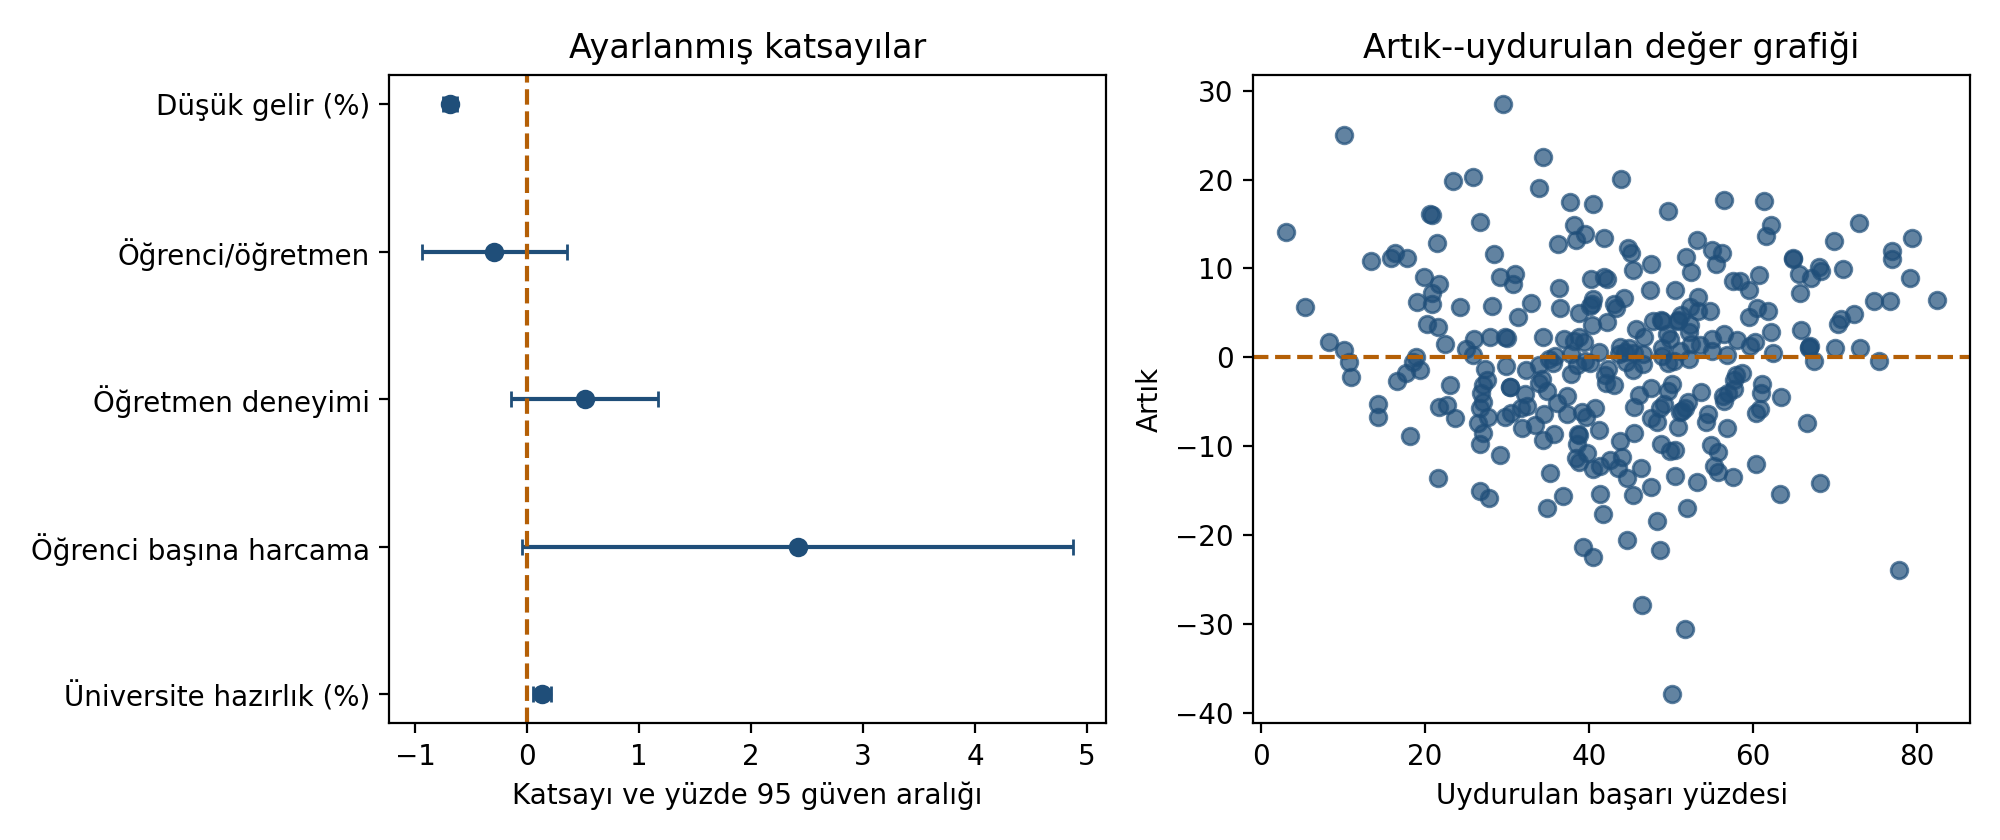
\includegraphics[width=\textwidth]{companion/outputs/figures/chapter15_multiple_regression.png}
\caption{STAR98 modelinde ayarlanmış katsayılar ve artık grafiği. Sol paneldeki katsayı büyüklükleri farklı ölçüm birimlerine dayandığından birbirleriyle doğrudan önem sıralamasına sokulmamalıdır.}
\label{fig:multiple-regression-diagnostics}
\end{figure}

Şekil~\ref{fig:multiple-regression-diagnostics}, katsayı aralıkları ile artık
tanısını aynı sayfada birleştirir; yorum ilkeleri Bölüm~\ref{sec:multiple-diagnostics}'te
verilen kontrollerle birlikte uygulanmalıdır.

\section{Yazılım uygulaması}

\begin{softwarebox}
\begin{lstlisting}
import pandas as pd
import statsmodels.api as sm
from statsmodels.stats.outliers_influence import (
    variance_inflation_factor)

data = pd.read_csv(
    "companion/data/clean/star98_districts.csv")

predictors = [
    "low_income_pct",
    "pupil_teacher_ratio",
    "teacher_experience_years",
    "spending_per_pupil_thousands",
    "college_prep_pct"
]
y = 100 * data["above_median_rate"]
X = sm.add_constant(data[predictors])
model = sm.OLS(y, X).fit()

print(model.summary())
print(model.conf_int())

for index, name in enumerate(predictors, start=1):
    vif = variance_inflation_factor(X.to_numpy(), index)
    print(name, vif)
\end{lstlisting}
Tam tablo ve grafikleri üreten betik
\path{companion/code/06_multiple_regression.py} dosyasındadır. Model
formülü, veri hazırlama adımları ve kullanılan değişkenler sonuçlarla birlikte
saklanmalıdır. Bu uygulamada kullanılan statsmodels altyapısı için bkz.
\citet{seabold2010}.
\end{softwarebox}

\begin{assumptionbox}
Regresyon katsayısı ancak modele alınan diğer açıklayıcılar sabitken yorumlanır.
Modelde bulunmayan karıştırıcılar, ölçüm hatası, örnekleme tasarımı ve yanlış
fonksiyonel biçim ayarlanmış katsayıyı yine yanıltabilir. Çok değişkenli model,
gözlemsel veriyi kendiliğinden deneysel veriye dönüştürmez.
\end{assumptionbox}

\begin{mistakebox}
Bir değişkenin \pval-değeri büyük diye modelden otomatik çıkarılması doğru değildir.
Değişken bilimsel olarak gerekli bir karıştırıcı olabilir. Tersine küçük
\pval-değeri de değişkenin nedensel, önemli veya iyi bir öngörücü olduğunu tek
başına göstermez.
\end{mistakebox}

\begin{outputguidebox}
Önce yanıt değişkenini, analiz birimini ve referans kategorileri belirleyin.
Ardından her katsayının işaretini, birimini, güven aralığını ve \pval-değerini
birlikte okuyun. Model düzeyinde $R^2$, düzeltilmiş $R^2$, genel \Fstat testi ve
artık standart hatasını; tanı aşamasında artık grafikleri, VIF ve etkili
gözlemleri inceleyin.
\end{outputguidebox}

\section{Çözümlü problemler}

\subsection*{Problem 1: Katsayı ve öngörü yorumu}

Bir model
\[
\hat Y=40+2X_1-3X_2
\]
biçimindedir. $X_1$ haftalık çalışma saati, $X_2$ devamsızlık günü olsun.
Katsayıları yorumlayın ve $X_1=5$, $X_2=2$ için öngörüyü bulun.

\textbf{Çözüm.} Aynı devamsızlık düzeyinde çalışma süresindeki bir saatlik
fark, ortalama iki puanlık daha yüksek $Y$ ile ilişkilidir. Aynı çalışma
süresinde bir günlük ek devamsızlık, ortalama üç puanlık daha düşük $Y$ ile
ilişkilidir. Öngörü
\[
\hat y=40+2(5)-3(2)=44
\]
olur. Sabit terim, çalışma ve devamsızlık sıfırken beklenen 40 puandır; bu
koşul veri aralığında değilse ayrı bir bağlamsal anlam taşımayabilir.

\subsection*{Problem 2: Basit ve ayarlanmış katsayı}

Düşük gelirli öğrenci yüzdesinin başarı yüzdesiyle basit regresyon katsayısı
$-0{,}748$, okul özellikleri eklendikten sonraki katsayısı $-0{,}685$'tir.
Bu değişimi yorumlayın.

\textbf{Çözüm.} Basit katsayı düşük gelir oranıyla başarı arasındaki toplam
doğrusal ilişkiyi özetler. Çoklu katsayı ise öğrenci--öğretmen oranı, öğretmen
deneyimi, harcama ve üniversite hazırlık oranı aynı tutulduğunda kalan koşullu
ilişkidir. Mutlak değerin 0,063 azalması, basit ilişkinin bir bölümünün bu okul
özellikleriyle ortak olduğunu düşündürür.

Katsayının değişmesi tek başına hangi değişkenin karıştırıcı olduğunu veya
nedensel yapının doğru kurulduğunu kanıtlamaz. Örnekleme değişkenliği,
ölçüm hatası ve model biçimi de karşılaştırmayı etkileyebilir.

\subsection*{Problem 3: Gösterge değişken yorumu}

\[
\hat Y=65+4\,\text{Program}-0{,}5\,\text{Devamsızlık}
\]
modelinde Program $=1$ uygulama, Program $=0$ karşılaştırma grubudur. Program
katsayısını ve beş gün devamsızlığı olan iki grup için öngörüleri yorumlayın.

\textbf{Çözüm.} Aynı devamsızlık düzeyinde uygulama grubunun beklenen puanı
karşılaştırma grubundan dört puan yüksektir. Beş günlük devamsızlık için
\[
\hat y_{\text{karşılaştırma}}=65-0{,}5(5)=62{,}5,
\]
\[
\hat y_{\mathrm{program}}=65+4-0{,}5(5)=66{,}5.
\]
Aradaki dört puanlık ayarlanmış fark bütün devamsızlık düzeylerinde aynıdır;
çünkü modelde etkileşim bulunmamaktadır.

\subsection*{Problem 4: Etkileşimli model}

\[
\hat Y=50+2X-3Z+1{,}5XZ
\]
modelinde $X$ çalışma süresi, $Z=1$ çevrim içi ve $Z=0$ yüz yüze öğretim
olsun. İki gruptaki çalışma süresi eğimlerini ve $X=4$ düzeyindeki grup
farkını bulun.

\textbf{Çözüm.} Yüz yüze grupta $Z=0$ olduğundan eğim 2'dir. Çevrim içi
grupta çalışma süresi eğimi
\[
2+1{,}5=3{,}5
\]
olur. Çevrim içi eksi yüz yüze grup farkı çalışma süresine bağlıdır:
\[
-3+1{,}5X.
\]
$X=4$ için fark $-3+1{,}5(4)=3$ puandır. Etkileşim bulunduğu için ``çevrim
içi öğretimin genel etkisi $-3$ puandır'' denemez; $-3$ yalnız $X=0$
düzeyindeki grup farkıdır.

\subsection*{Problem 5: Düzeltilmiş açıklanan varyans}

$n=100$, $p=4$ ve $R^2=0{,}40$ olan bir modelin düzeltilmiş $R^2$ değerini
hesaplayın.

\textbf{Çözüm.}
\[
R^2_{\mathrm{düz}}
=1-(1-0{,}40)\frac{100-1}{100-4-1}
=1-0{,}60\frac{99}{95}
\approx0{,}375.
\]
Düzeltilmiş değer 0,40'tan küçüktür; çünkü dört açıklayıcının modele getirdiği
uyum artışı model karmaşıklığına göre cezalandırılmıştır. Bu değer yeni
verideki öngörü başarısının garantisi değildir; dış doğrulama veya çapraz
doğrulama ayrı değerlendirilmelidir.

\subsection*{Problem 6: Gerçek model çıktısını bütüncül yorumlama}

STAR98 modelinde $R^2=0{,}724$, düzeltilmiş $R^2=0{,}719$,
$F(5,297)=155{,}72$, $p<0{,}001$; düşük gelir katsayısı
$-0{,}685$ ve güven aralığı $[-0{,}746;-0{,}624]$ bulunmuştur. VIF değerleri
1,27--1,73 arasındadır. Sonucu yorumlayın.

\textbf{Çözüm.} Model, okul bölgelerinin başarı yüzdelerindeki örneklem
değişkenliğinin yaklaşık yüzde 72,4'ünü açıklamaktadır. Düzeltilmiş değerin
çok yakın olması beş açıklayıcının oluşturduğu karmaşıklık cezasının küçük
olduğunu gösterir. Genel \Fstat testi, açıklayıcıların birlikte doğrusal bilgi
taşıdığına ilişkin güçlü kanıt verir.

Diğer açıklayıcılar sabitken düşük gelir oranındaki bir yüzde puanlık fark,
başarı oranında ortalama 0,685 yüzde puanlık ters yönlü farkla ilişkilidir.
Güven aralığının tamamı negatiftir. VIF değerleri bu değişken kümesinde güçlü
çoklu bağlantı işareti vermemektedir. Buna rağmen model bölge düzeyinde ve
gözlemseldir; bireysel öğrenciler veya nedensel etkiler hakkında doğrudan
sonuç çıkarılamaz.

\section{R ile çözümlü uygulama}
\label{sec:r-multiple}

\textbf{Soru.} Bölümdeki $40+2X_1-3X_2$ modelini, açıkça yapay olarak
oluşturulan 12 satırlık bir öğretim verisi üzerinde tahmin edin. Ayarlanmış
katsayıları, $R^2$'yi, VIF değerlerini ve beş saat çalışma ile iki gün
devamsızlık için öngörüyü bulun. Bu veri gerçek okul bölgesi verisi değildir.

\begin{lstlisting}[style=prismR]
veri <- expand.grid(saat = c(2, 4, 6, 8),
                     devamsizlik = c(0, 1, 2))
hata <- c(1, -1, -1, 1, -2, 2, 2, -2, 1, -1, -1, 1)
veri$puan <- 40 + 2 * veri$saat -
  3 * veri$devamsizlik + hata
model <- lm(puan ~ saat + devamsizlik, data = veri)
summary(model)
confint(model)
yardimci_saat <- lm(saat ~ devamsizlik, data = veri)
yardimci_devam <- lm(devamsizlik ~ saat, data = veri)
c(VIF_saat = 1 / (1 - summary(yardimci_saat)$r.squared),
  VIF_devamsizlik =
    1 / (1 - summary(yardimci_devam)$r.squared))
yeni <- data.frame(saat = 5, devamsizlik = 2)
predict(model, newdata = yeni, interval = "confidence")
predict(model, newdata = yeni, interval = "prediction")
plot(fitted(model), resid(model),
     xlab = "Uydurulan deger", ylab = "Artik")
abline(h = 0, lty = 2)
qqnorm(resid(model))
qqline(resid(model))
\end{lstlisting}

\begin{outputguidebox}
\textbf{Çözüm ve kontrol değerleri.} Katsayılar sırasıyla 40, 2 ve
$-3$; $R^2=0{,}9286$ ve düzeltilmiş $R^2=0{,}9127$'dir. Her iki VIF
1'dir; tasarlanan açıklayıcılar doğrusal olarak ilişkisizdir. Beş saat ve
iki gün için öngörü $40+2(5)-3(2)=44$ puandır. Saat katsayısının model-temelli
yüzde 95 güven aralığı yaklaşık $[1{,}5231;2{,}4769]$'dur.
\end{outputguidebox}

\textbf{Yorum.} Aynı devamsızlıkta bir saatlik fark, modelde iki puanlık
beklenen farkla ilişkilidir. Yapay hata dizisi katsayıları kolay kontrol
edebilmek için seçilmiştir; elde edilen $p$ ve güven aralıkları gerçek bir
evrene ilişkin kanıt değildir. Gerçek çıkarımda hata modeli ve örnekleme
tasarımı ayrıca gerekçelendirilir. VIF'nin küçük olması bu varsayımları doğrulamaz.

\textbf{Pekiştirme ve yanıt.} Aynı beş saatte devamsızlık bir güne inerse
öngörü 47 olur. Üç puanlık koşullu farkı otomatik olarak nedensel etki saymayın.

\section{Tamamlayıcı vaka: hangi ortalama, kimin oranı?}
\label{sec:v4-star98}

\textbf{Soru ve kapsam.} STAR98'in aynı sayımlarıyla iki soru soralım:
``Dosyadaki bölgelerin oran ortalaması nedir?'' ve ``Bu sayımlarda temsil
edilen öğrencilerin toplam üst kategori oranı nedir?'' Yeni bir regresyon
kurmayacağız; özetlenen hedefin neden değiştiğini inceleyeceğiz.

Dağıtıcının açıklaması satırları birleşik okul bölgesi, yanıtı 9. sınıf
matematik sonuçlarının sayımı olarak tanımlar; dosya özgün kaynağın alt
kümesidir. Aynı sayfanın notlarında geçen \textit{counties} ifadesiyle
adlandırma çelişkisi çözülmüş değildir. Burada ``bölge'', açıklamadaki
tanıma dayanır; gerçek coğrafi kimlikler bağımsız doğrulanmış sayılmaz.\footnote{Dağıtıcı tanımı:
\url{https://www.statsmodels.org/stable/datasets/generated/star98.html};
erişim 13 Eylül 2026. Kaynak eser: \citet{gill2001}.}

\textbf{Analiz tanımı.} Yerel 303 satırın tamamı kullanılır. $a_j$, kaynakta
\texttt{NABOVE}; $b_j$, \texttt{NBELOW}; $n_j=a_j+b_j$ ve $r_j=a_j/n_j$
olsun. Üst kategori kaynağın ulusal medyan üstü tanımıdır; medyana eşit
puanların işlemine ilişkin yeni bir kural varsayılmaz. Payda bütün kayıtlı
öğrenciler değil, bu iki sayımın toplamıdır. Kimlik yerel sıra anahtarıdır.
Eksik, negatif, kesirli sayım veya sıfır payda varsa işlem durur; otomatik
silme ya da doldurma yapılmaz. Sıfır üst sayımı ise geçerlidir.

\subsection*{İki hedefi hesaplamadan önce tanımlayın}

$J=303$ için eşit bölge ağırlıklı özet
\[
\bar r_{\mathrm{bölge}}=\frac{1}{J}\sum_{j=1}^{J}r_j
\]
her satıra $1/J$ ağırlığı verir. Toplam sayım oranı ise
\[
r_{\mathrm{toplam}}=\frac{\sum_j a_j}{\sum_j n_j}
=\sum_j\frac{n_j}{\sum_k n_k}r_j
\]
olup satırları sayım büyüklükleriyle ağırlıklandırır. Her iki formül de
aynı kayıtların betimlemesidir; ikinci formülün ağırlıkları ters dahil
edilme olasılığı değildir. Büyük bölgeye daha fazla ağırlık vermek,
kendiliğinden örnekleme yanlılığını düzeltmez.

\begin{table}[H]
\centering
\small
\caption{V4: aynı 303 kayıtta iki farklı hedef}
\label{tab:v4-hedefler}
\begin{tabularx}{\linewidth}{@{}Xr@{}}
\toprule
Özet & Değer \\
\midrule
Üst kategori toplamı & 108\,418 \\
İki kategorinin toplamı & 267\,611 \\
Eşit bölge ağırlıklı oran (yüzde) & 43,697840 \\
Toplam sayım oranı (yüzde) & 40,513282 \\
Toplam eksi bölge özeti (yüzde puan) & $-3{,}184558$ \\
\bottomrule
\end{tabularx}
\end{table}

Kayıt başına toplam 33 ile 38\,852 arasında değişir. Bu veride büyüklükle
ağırlıklandırılmış oran daha düşüktür. Bu fark bir yazılım uyuşmazlığı
değildir; hedef değişmiştir. Her büyük bölgenin oranının her küçük
bölgeden düşük olduğu sonucu da çıkmaz. B11--B12'de soru değişince
ortalama ve oran ayrılıyordu; burada değişken aynı kalırken ağırlıklandırma
hedefi değişmektedir.

\noindent\begin{minipage}{\linewidth}
\textbf{Yeniden üretim.} Proje kökünden, yalnız betimsel iki özeti hesaplayın:
\begin{lstlisting}[style=prismPythonApp]
import pandas as pd

data = pd.read_csv(
    "companion/data/raw/star98_statsmodels.csv")
counts = data[["NABOVE", "NBELOW"]]
assert len(data) == 303
assert data["DISTRICT_ID"].is_unique
assert counts.notna().all().all()
assert (counts >= 0).all().all()
assert (counts % 1 == 0).all().all()
total = counts.sum(axis=1)
assert (total > 0).all()
rate = counts["NABOVE"] / total
equal_rate = rate.mean()
pooled_rate = counts["NABOVE"].sum() / total.sum()
print(100 * equal_rate, 100 * pooled_rate)
print(100 * (pooled_rate - equal_rate))
\end{lstlisting}
\end{minipage}

Kaynak hash'i, yerel anahtar ve ham--temiz aktarım denetimi dahil tam kod
\path{companion/vakalar/v4-star98/analyze.py} dosyasındadır.
Bu özetler için güven aralığı veya \pval-değeri üretilmez: dosyanın
betimlenmesi, özgün örnekleme mekanizmasının ya da öğrencilerin bağımsız
Bernoulli gözlemleri olduğunun doğrulanması değildir. 267\,611 sayısını
bağımsız örneklem büyüklüğü sayıp otomatik binom aralığı hesaplamayın.

\subsection*{Toplulaştırma hangi bilgiyi kaybettirir?}

Aşağıdaki iki tablo \textbf{tamamen yapaydır}; STAR98'in bireyleri değildir.
Her senaryoda 100 kişi, 50 düşük gelirli kişi ve toplam 50 üst kategori
sonucu vardır. Yine de grup içi ilişkiler ters yöndedir.

\begin{table}[H]
\centering
\small
\caption{Aynı marjinleri veren iki yapay bireysel düzen}
\label{tab:v4-yapay}
\begin{tabular}{@{}llrr@{}}
\toprule
Senaryo & Grup & Üst & Alt \\
\midrule
A & Düşük gelir & 40 & 10 \\
A & Diğer & 10 & 40 \\
B & Düşük gelir & 10 & 40 \\
B & Diğer & 40 & 10 \\
\bottomrule
\end{tabular}
\end{table}

İki senaryoda da düşük gelir oranı ve üst kategori oranı \%50'dir. Fakat
düşük gelir eksi diğer grup oran farkı A'da $0{,}8-0{,}2=0{,}6$,
B'de $0{,}2-0{,}8=-0{,}6$ olur. Yalnız marjinleri bilmek bireysel
ilişkiyi belirlemez. Bölümdeki bölgesel regresyon katsayısını bireysel gelir
etkisi sayamayız. Bu gösterim gerçek STAR98'de bir terslenme kanıtı değildir;
toplulaştırmanın hangi bilgiyi sakladığını gösterir. B13'ün öğrenci düzeyi
uygulamasında birim farklıdır; veri dosyaları birleştirilmez.

\subsection{Görevler, kontrol yanıtları ve puanlama}

Her görev iki bileşenlidir; her bileşen 1 puan, toplam \textbf{10 puan}.
Önce yanıtınızı yazın, sonra aşağıdaki gerekçelerle karşılaştırın.
\begin{enumerate}
\item Bir satırın birimini ve toplam sayım oranının paydasını tanımlayın.
  267\,611 sayısı hangi evreni otomatik olarak temsil etmez?
\item İki oranın neden farklı olduğunu ağırlıklarıyla açıklayın.
  ``Büyük olan doğru, küçük olan hatalı'' yorumunu değerlendirin.
\item $n_j/\sum_k n_k$ ağırlığının örnekleme ağırlığı olup olmadığını
  tartışın. Toplam sayımdan neden hemen bir binom güven aralığı üretmiyoruz?
\item Yapay A ve B'de düşük gelir eksi diğer grup oran farkını bulun.
  Aynı marjinlerden bireysel ilişkinin neden belirlenemediğini açıklayın.
\item İki gerçek özeti içeren, genelleme ve nedensellik sınırları açık
  kısa bir rapor yazın. Yapay kişileri gerçek toplamın dışında tutun.
\end{enumerate}

\textbf{Gerekçeli kontrol yanıtları.}
\begin{enumerate}
\item Satır, dağıtıcı açıklamasındaki bölge düzeyi toplulaştırmadır;
  payda iki kayıtlı sonuç sayısının toplamıdır (1). Kaynak alt kümesi,
  bütün California/ABD öğrencilerinin evreni değildir; idari adlandırma
  çelişkisi ayrıca korunur (1).
\item Birinci özet her satıra $1/303$, ikinci özet sayım büyüklüğüyle
  orantılı ağırlık verir (1). Hedefler farklı olduğundan fark hata veya
  üstünlük kanıtı değildir; rapor soruya uygun hedefi belirtmelidir (1).
\item Bunlar büyüklük ağırlıklarıdır; dahil edilme olasılıkları
  belgelenmiş değildir (1). Bireysel bağımsızlık ve örnekleme modeli
  kurulmadığından toplam sayı doğrudan binom belirsizliğini haklı kılmaz (1).
\item A'da $+0{,}6$, B'de $-0{,}6$ (60 ve eksi 60 yüzde puan) bulunur (1).
  Aynı marjinlerle zıt ilişkiler mümkün olduğundan bireysel ilişki
  belirlenemez; bunun gerçek terslenme kanıtı olmadığı belirtilir (1).
\item Rapor iki özeti doğru adlarıyla verir ve yapay tabloları gerçek
  hesaplara katmaz (1). Örnekleme kapsamını aşan genelleme ve bireysel
  nedensellik kurmaz (1); doğru sayılar tek başına tam puan getirmez.
\end{enumerate}

\textbf{Kısa rapor örneği.} ``Yerel STAR98 dosyasındaki 303 toplulaştırılmış
kayıtta eşit bölge ağırlıklı üst kategori oranı ortalaması \%43,697840;
108\,418 üst sayımın 267\,611 toplam sayıma oranı \%40,513282'dir.
Fark ağırlıklandırma hedefinden kaynaklanır. Sonuçlar bu kayıtları betimler;
tüm öğrenciler için evren tahmini veya bireysel gelir etkisi değildir.
Örnekleme belirsizliği bu betimsel karşılaştırmada hesaplanmamıştır.''

\begin{etkinlik}
Modeli üç düzeyde denetleyin: (1) katsayıların birimi ve referans kategorisi,
(2) artık, doğrusal biçim, varyans ve etkili gözlem tanıları, (3) ayarlama
kümesinin araştırma sorusuna ve olası nedensel yapıya uygunluğu.
\end{etkinlik}

\section{Bölüm özeti}

\begin{itemize}
  \item Çoklu regresyon katsayısı diğer modele alınmış açıklayıcılar sabitken yorumlanır.
  \item Katsayıların değişmesi ortak bilgi veya karıştırıcılık olasılığını gösterebilir.
  \item Kategorik açıklayıcılar referans kategoriye dayalı göstergelerle temsil edilir.
  \item Etkileşim, bir açıklayıcının eğiminin başka bir değişkene göre değişmesidir.
  \item Düzeltilmiş $R^2$ model karmaşıklığını dikkate alır; genel \Fstat testi model düzeyinde kanıt verir.
  \item VIF, artık grafikleri ve etkili gözlem tanıları katsayı yorumunun parçasıdır.
\end{itemize}

\bolumkaynaklari{\cite{gelman2020,fox2016,james2021}}

\section*{Alıştırmalar}

\begin{enumerate}
  \item Basit ve çoklu regresyon katsayılarının yanıtladığı soruları karşılaştırın.
  \item ``Diğer değişkenler sabitken'' ifadesinin anlamını açıklayın.
  \item $\hat Y=30+4X_1-2X_2$ modelinde $X_1=3$, $X_2=5$ için öngörü yapın.
  \item Bir katsayının modele yeni değişken eklendiğinde neden değişebileceğini açıklayın.
  \item Üç kategorili okul türü değişkeni için kaç gösterge gerektiğini ve referansın rolünü yazın.
  \item Gösterge değişken katsayısı $-6$ ise uygun bir bağlamsal yorum oluşturun.
  \item $Y=\beta_0+\beta_1X+\beta_2Z+\beta_3XZ$ modelinde $Z=0$ ve $Z=1$ için eğimleri yazın.
  \item Etkileşimli modelde ana etkilerin neden tek başına genel etki olmadığını açıklayın.
  \item Merkezlemenin sabit terim yorumunu nasıl değiştirdiğini belirtin.
  \item $n=80$, $K=5$ ve $R^2=0{,}50$ için düzeltilmiş $R^2$ değerini hesaplayın.
  \item Genel \Fstat testi anlamlı, tek katsayıların bazıları anlamsızsa sonucu yorumlayın.
  \item Bir değişken için $R_j^2=0{,}80$ ise VIF değerini hesaplayın.
  \item Yüksek VIF'nin katsayı ve standart hata üzerindeki olası etkilerini açıklayın.
  \item Artık grafiğindeki eğri ve huni örüntülerini model sorunlarıyla eşleştirin.
  \item Çoklu regresyonun gözlemsel veride neden otomatik nedensellik sağlamadığını açıklayın.
  \item Model seçimini yalnız \pval-değerlerine dayandırmanın iki sakıncasını yazın.
\end{enumerate}